\section{Multilayer Perceptron}

\subsection{Methods}
This section covers how we went about implementing the MLP back-progagation gradient descent algorithm and which parameters we chose to make to make it perform well on the validation set.

\subsubsection{Treatment of Data}
First of all, before passing it on to the algorithm and training, we had to process the raw data of labelled digits.
\paragraph{Splitting}
The data was already separated into training and test data containing the pattern vectors for the digits and the corresponding classification labels. All what was left to do according to the instructions received was to split the training data into a random $\frac{2}{3}$ training and a $\frac{1}{3}$ validation set. This was easily achieved by randomly permuting the indices of the training data patterns and then dividing both the set of patterns and the set of labels at the $\frac{2}{3}$ mark according to the permutation.
\paragraph{Preprocessing}
Before starting off with training the MLP it had to be ensured that both training and validation set were properly normalized. As given in the project description, we computed the min. and max. values for every component of the untouched training patterns beforehand and then applied the normalization to the training and the test data. This preprocessing was actually done before splitting the data in order to save the operation on the validation set.

\subsubsection{MLP setup}
The structure of the MLP we were advised to use through the project instructions is depicted in Fig. ~\ref{fig:mlp}. The differences to the two-layer MLP discussed in the lecture lie in the following properties: Firstly, the first hidden layer has double the outputs than a "normal" MLP perceptron. Secondly, the gating function $g(a_{2k-1}, a_{2k})=a_{2k-1}\sigma(a_2k)$ takes pairs of values from the hidden layer accordingly. Lastly, the activation value $a^{(2)}$ is not passed through another gating function.
\begin{figure}[!h]
	\centering
	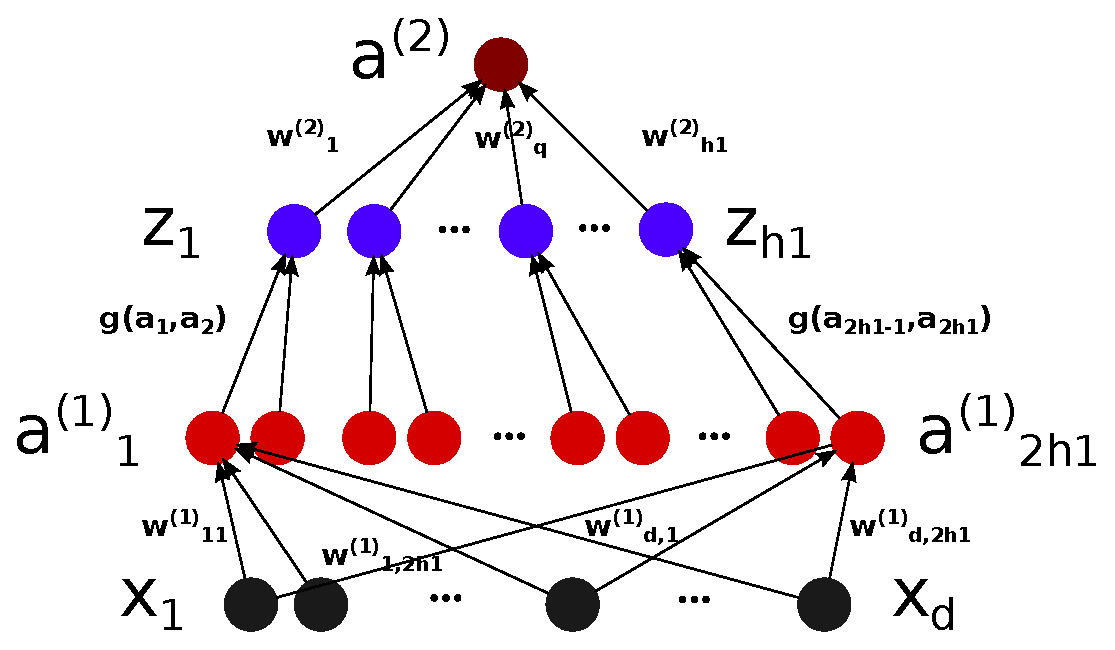
\includegraphics[width=.6\textwidth]{mlp/mlp.eps}
	\caption{Schema of the MLP described in the project instructions}
	\label{fig:mlp}
\end{figure}
Once we had the code for this setup running in python, we left the number of hidden layers and the gating function untouched and proceeded with the optimization of the remaining parameters, the number of hidden inputs $h_1$, the learning rate $\eta$ and the momentum term $\mu$. The discussion of the effects of the adjustment of these parameters is discussed with early stopping meaning that the optimization stops as soon as the validation error starts increasing. The 0/1 errors displayed in the graphs of this section are always specific to the respective validation set. The graphs in this section were generated on the 3/5 subtask.
%\paragraph{Early stopping}
%Evaluate empirical error $\hat{R}(\hat{f};\mathcal{D}_V)$ for validation set $\mathcal{D}_V$ along-side the training-error $\hat{R}(\hat{f};\mathcal{D}_T)$while training the MLP on $\mathcal{D}_T$. Stop at the training at the epoch where the validation error stops decreasing and starts increasing. 
%Show comparative plots illustrating the effects of learning rate, number of hidden units, momentum, etc. on\\
\paragraph{Effects of parameters on convergence speed and errors}
\begin{itemize}
		\begin{figure}[!ht]
		\centering
		\begin{subfigure}[b]{.45\textwidth}
		\centering
		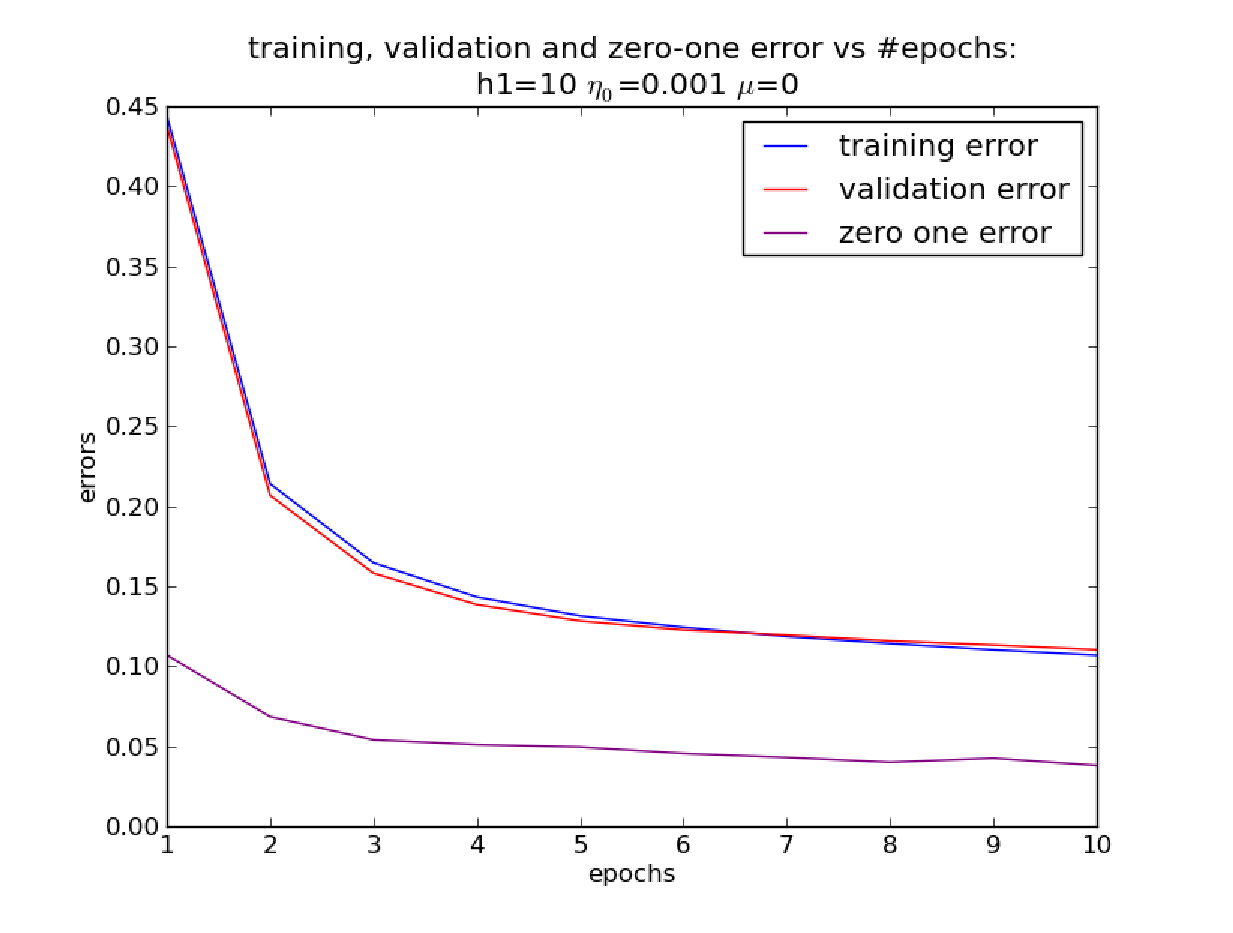
\includegraphics[width=\textwidth]{mlp/plots/effects/very_small_eta.eps}
		\caption{Errors with small $\eta_0=0.001$}
		\label{fig:small_eta}
		\end{subfigure}
		\quad
		\begin{subfigure}[b]{.45\textwidth}
		\centering
		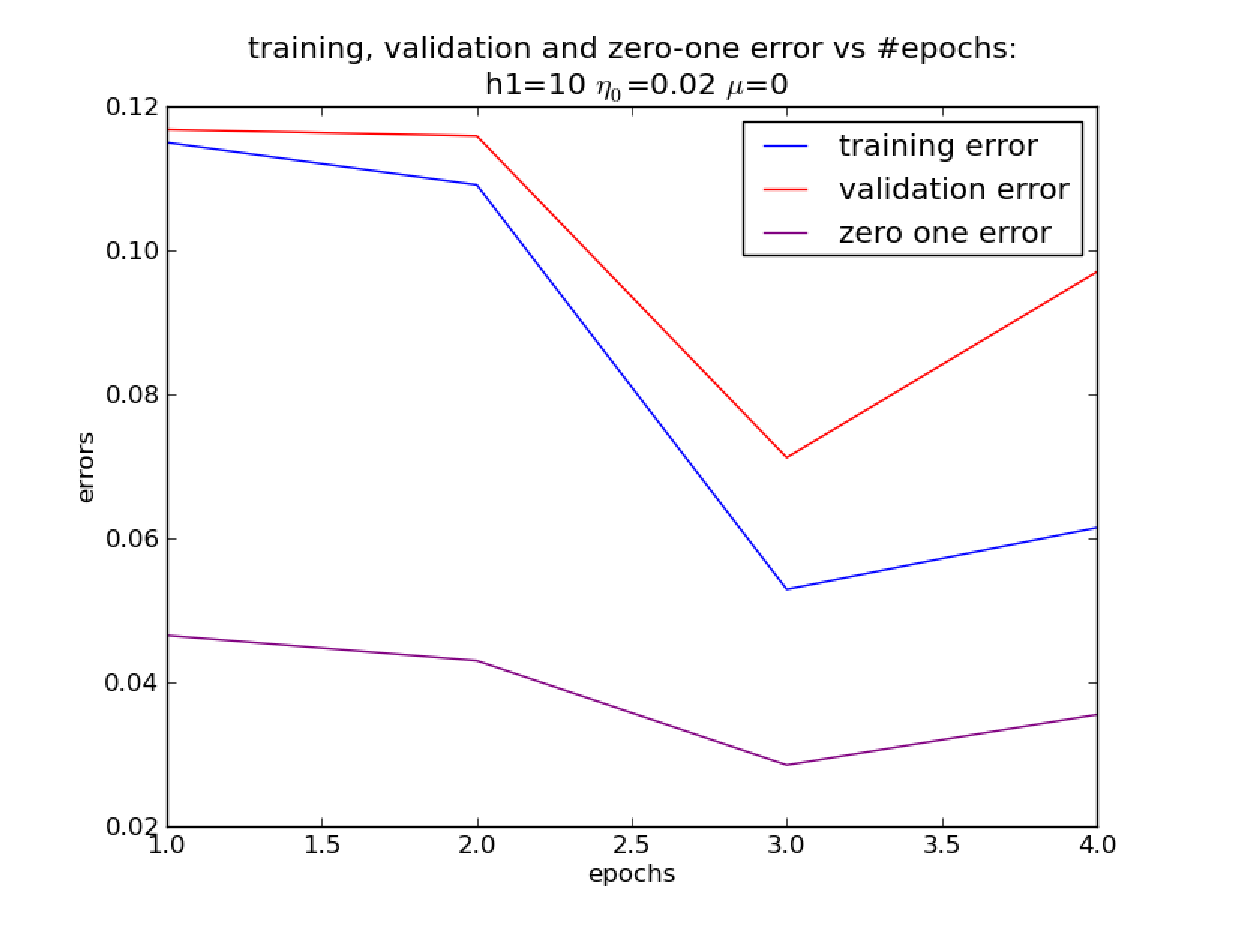
\includegraphics[width=\textwidth]{mlp/plots/effects/larger_eta.eps}
		\caption{Errors decrease with larger $\eta_0=0.02$}
		\label{fig:larger_eta}
		\end{subfigure}
		\begin{subfigure}[b]{.45\textwidth}
		\centering
		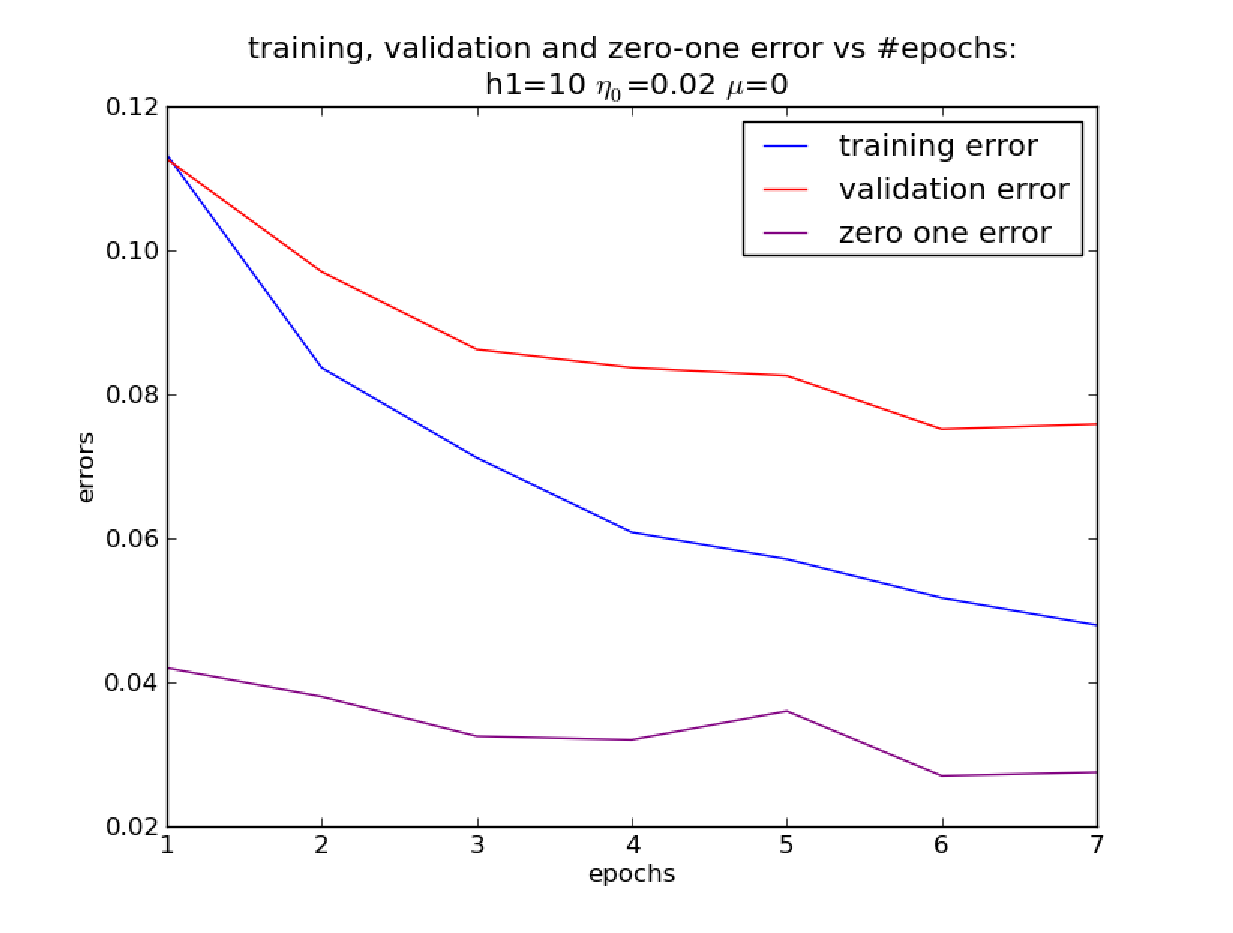
\includegraphics[width=\textwidth]{mlp/plots/effects/larger_eta_decrease.eps}
		\caption{Decreasing $\eta$ to $\eta=\frac{\eta_0}{epochs}$ after every epoch}
		\label{fig:decrease_eta}
		\end{subfigure}
		\quad
		\begin{subfigure}[b]{.45\textwidth}
		\centering
		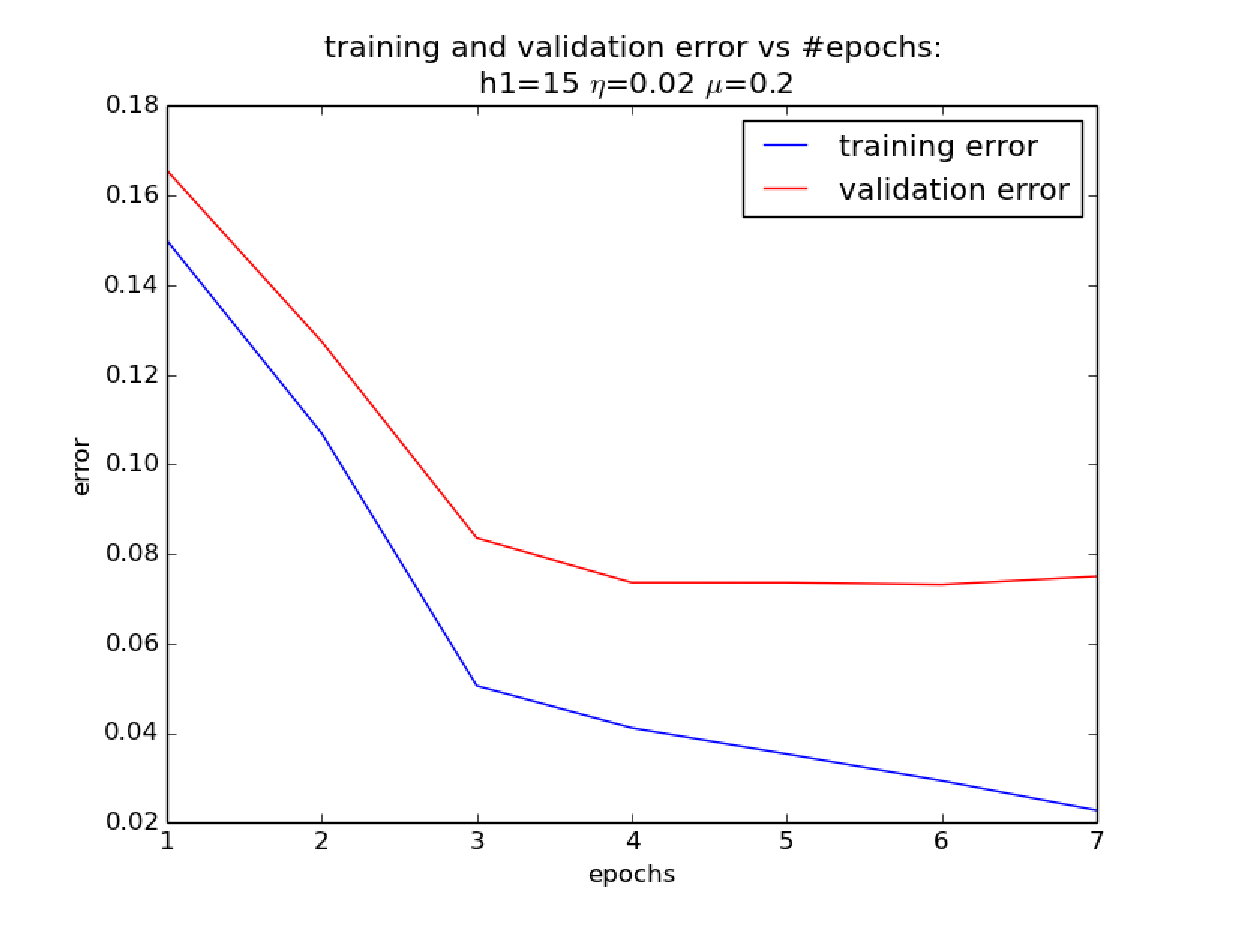
\includegraphics[width=\textwidth]{mlp/plots/effect_momentum.eps}
		\caption{Errors after introducing momentum term}
		\label{fig:increase_momentum}
		\end{subfigure}
		\caption{This figure exemplifies the effects of increasing the initial learning rate $\eta_0$ and then decreasing it every epoch, as well as the effect of introducing a momentum term stabilizing the gradient descent.}
		\label{fig:effects_learning_rate}
		\end{figure}
	\item In fig. \ref{fig:effects_learning_rate} we show the effects of the learning rate $\eta$ and the momentum term $\mu$ on the convergence speed and the accuracy of the MLP classifier. By increasing the initial learning rate $\eta_0$ we were able to decrease the number of epochs until an increase in the validation error occurs and improve the validation error. After decreasing the learning rate in every epoch, the optimization again takes a some epochs more to converge. Introducing a standard momentum term $\mu = 0.2$ as in fig. \ref{fig:increase_momentum} doesn't improve the convergence speed or the error values in our case. Before the decreasing the $\eta$ term in the manner depicted in subfig. caption \ref{fig:decrease_eta} we used momentum terms around $0.2$. Generally a higher learning rate makes the algorithm converge faster, this effect is increased by introducing the momentum term which is the decay-term for averaging the previous the gradients.  

	\item Effects of number hidden units $h_1$
		\begin{figure}[!ht]
		\begin{subfigure}[b]{.4\textwidth}
		\centering
		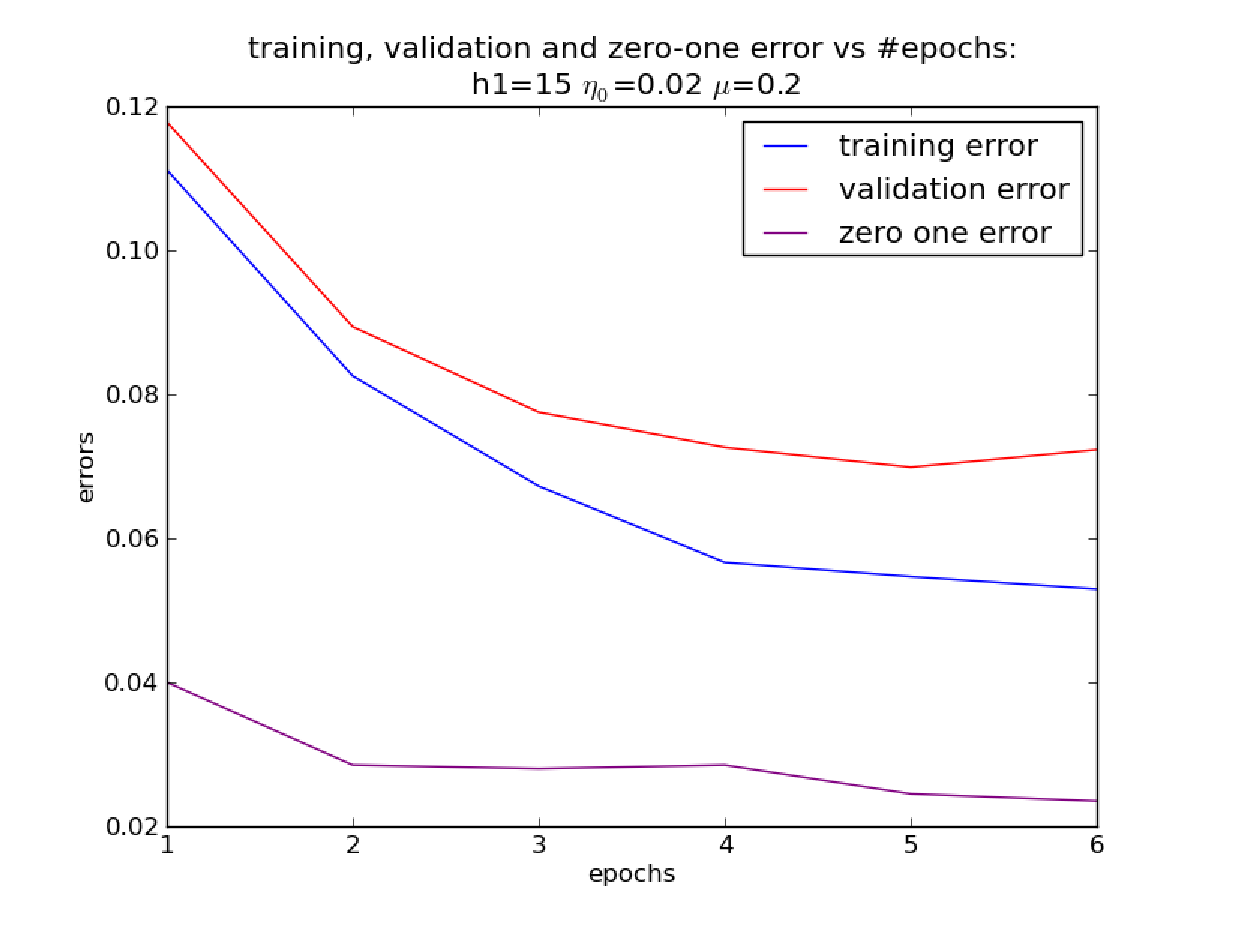
\includegraphics[width=\textwidth]{mlp/plots/effects/15h1.eps}
		\caption{$h_1=15$}
		\label{fig:h115}
		\end{subfigure}
		\centering
		\begin{subfigure}[b]{.4\textwidth}
		\centering
		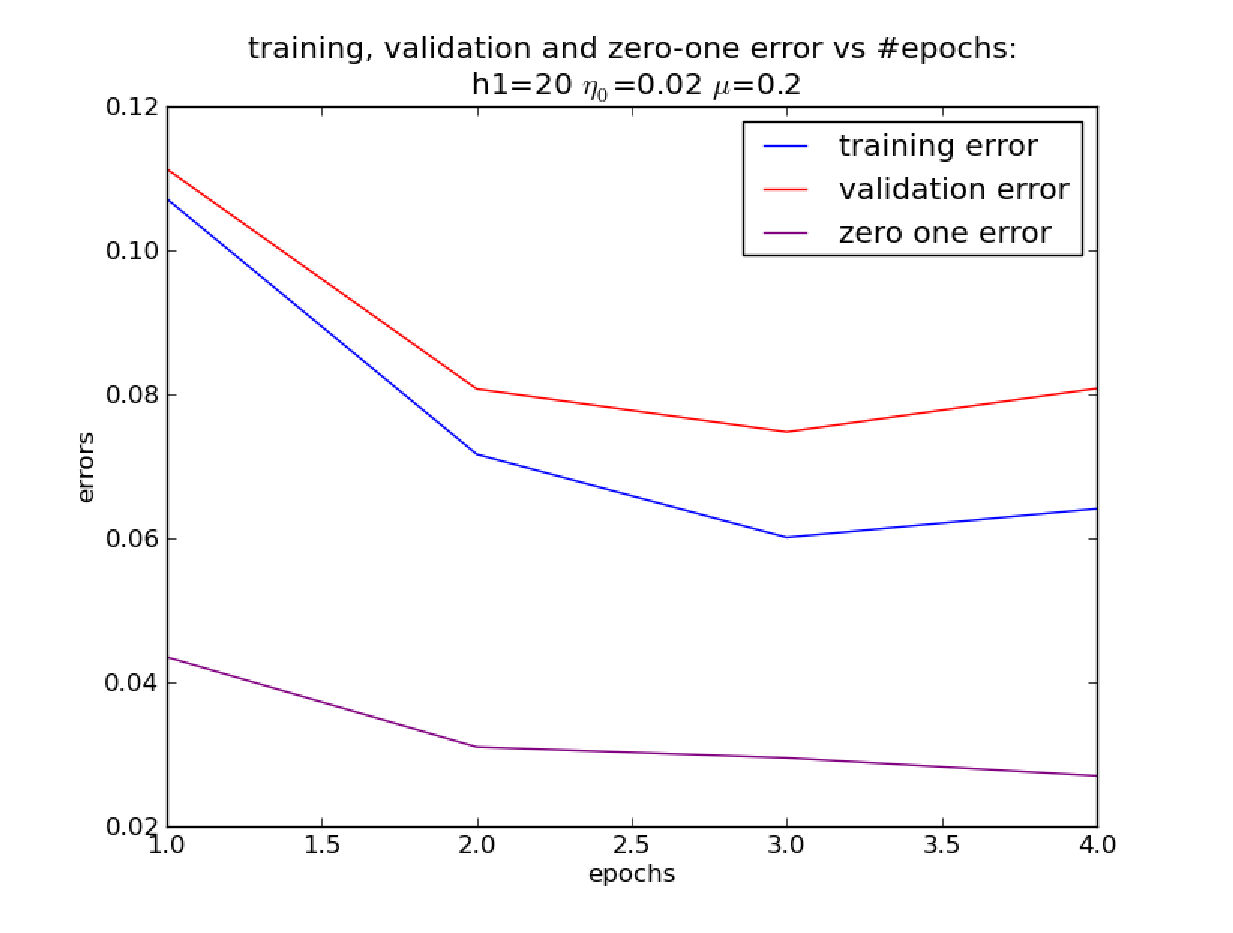
\includegraphics[width=\textwidth]{mlp/plots/effects/20h1.eps}
		\caption{$h_1=20$}
		\label{fig:h120}
		\end{subfigure}
		\quad
		\begin{subfigure}[b]{.4\textwidth}
		\centering
		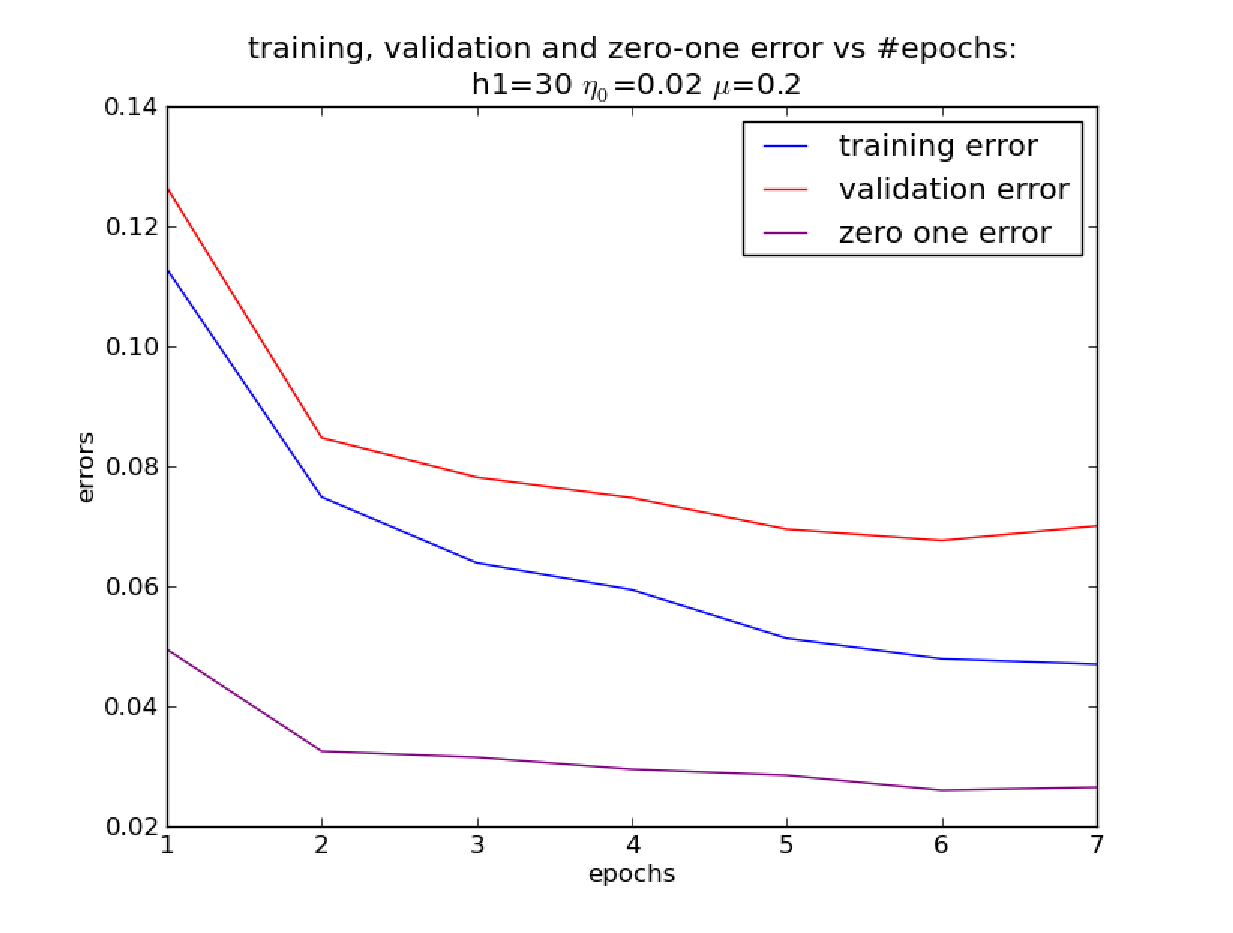
\includegraphics[width=\textwidth]{mlp/plots/effects/30h1.eps}
		\caption{$h_1=30$}
		\end{subfigure}
		\label{fig:h130}
		\quad
		\begin{subfigure}[b]{.4\textwidth}
		\centering
		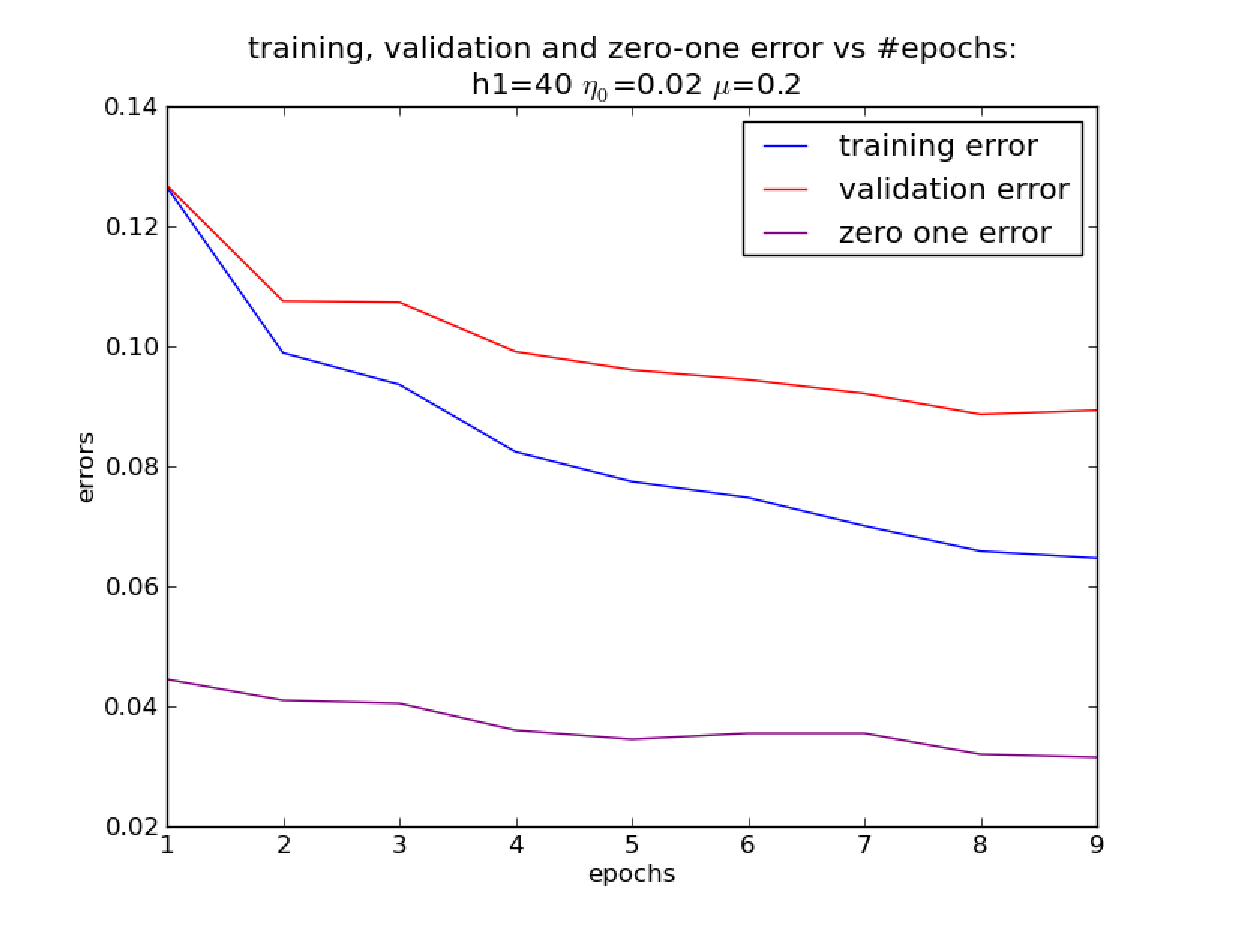
\includegraphics[width=\textwidth]{mlp/plots/effects/40h1.eps}
		\caption{$h_1=40$}
		\end{subfigure}
		\label{fig:h140}
		\quad
		\begin{subfigure}[b]{.4\textwidth}
		\centering
		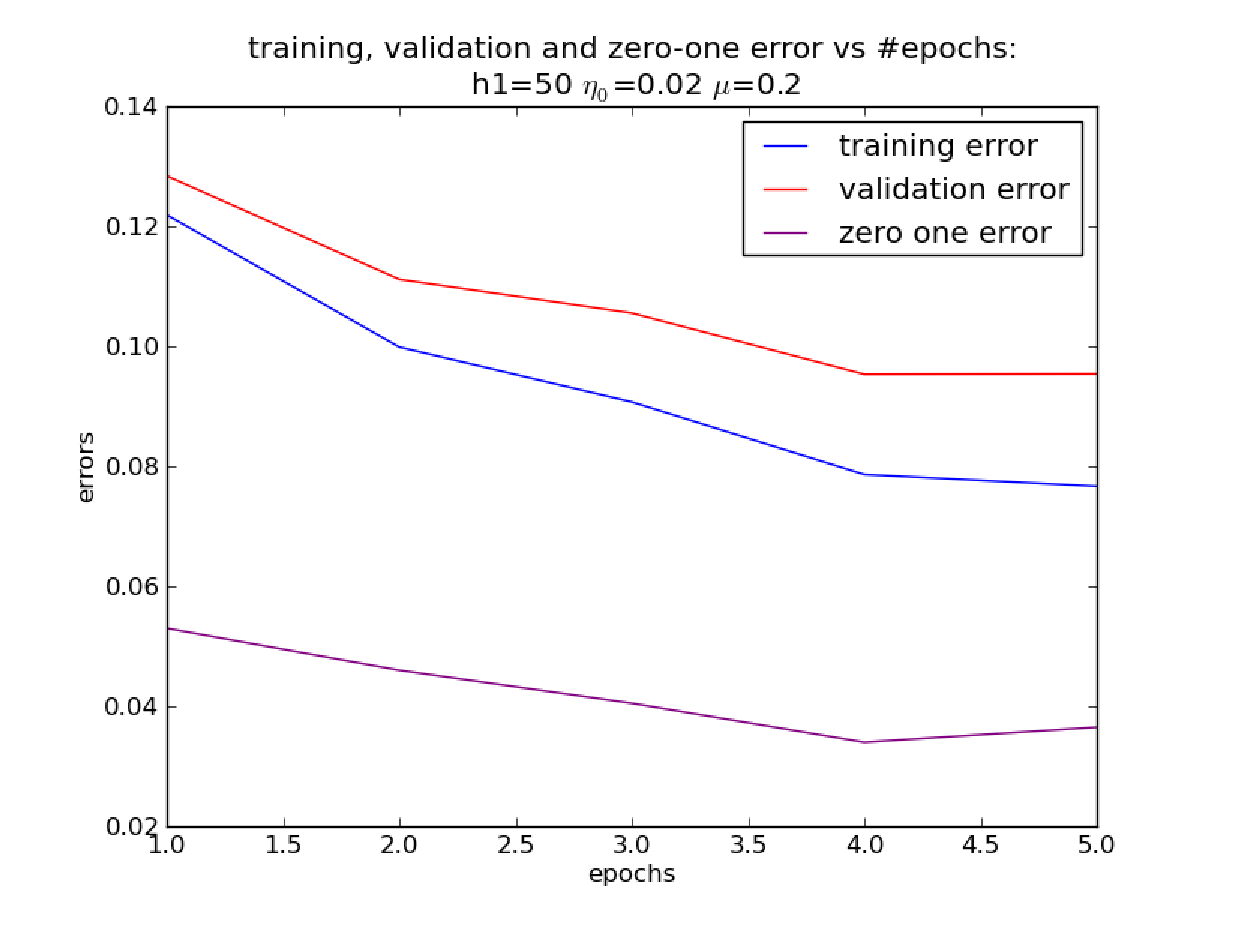
\includegraphics[width=\textwidth]{mlp/plots/effects/50h1.eps}
		\caption{$h_1=50$}
		\end{subfigure}	
		\label{fig:h150}
		\begin{subfigure}[b]{.4\textwidth}
		\centering
		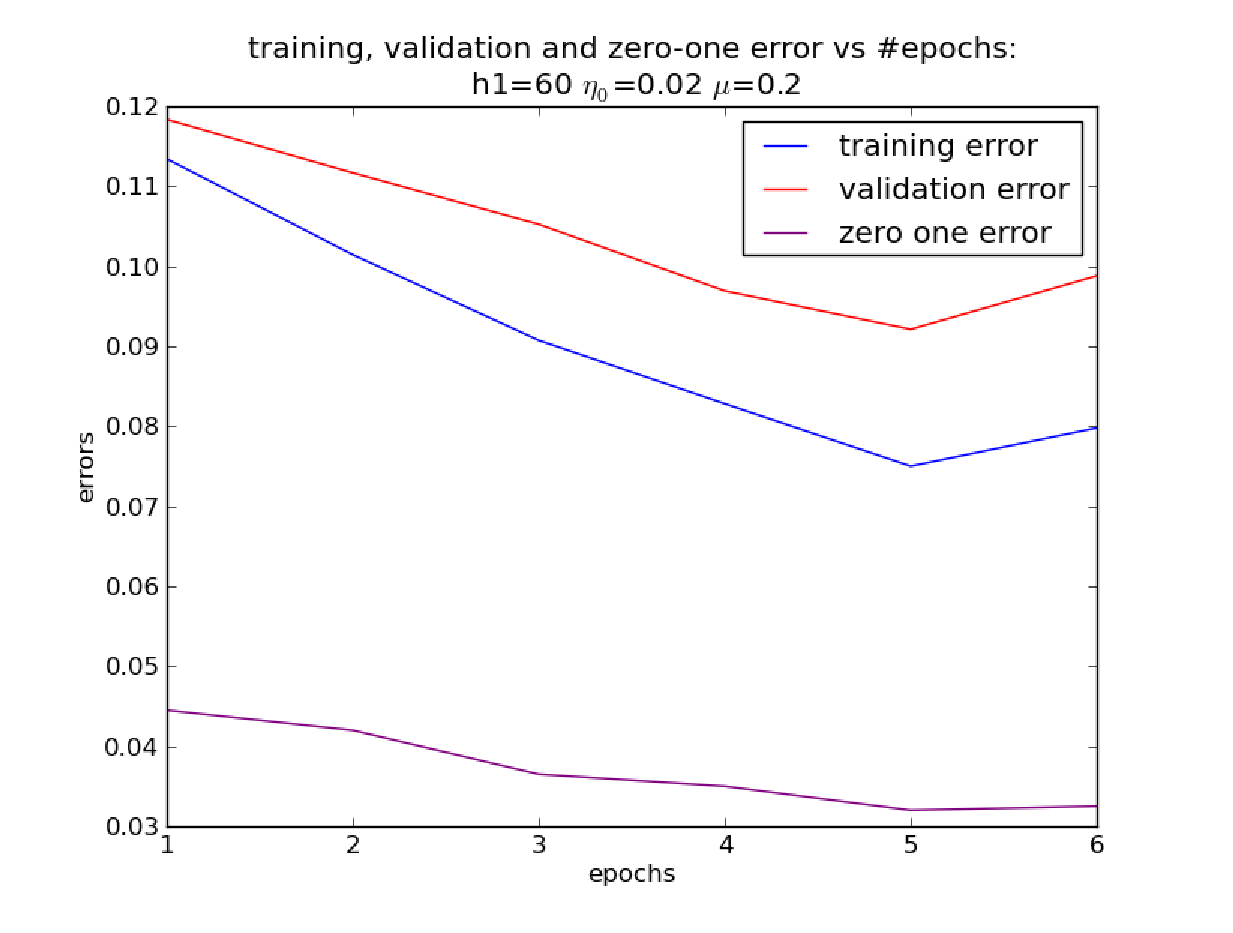
\includegraphics[width=\textwidth]{mlp/plots/effects/60h1.eps}
		\caption{$h_1=60$}
		\label{fig:h160}
		\end{subfigure}	
		\caption{Plotting graphs of the logistical error for different numbers of hidden units shows different performances and convergence in different numbers of epochs. No general pattern emerged in the depicted plots generated with early stopping. However, the model complexity should increase with the number of hidden units leading to an overfitting of the training set. More on this in the next section.}
		\label{fig:effects_h1}
		\end{figure}

\end{itemize}

\subsubsection{Effects of parameter choice on overfitting}
	\begin{figure}[!ht]
	\centering
	\begin{subfigure}[b]{.45\textwidth}
	\centering
	\includegraphics[width=\textwidth]{mlp/plots/test/15h1_overfitting_50_epochs.eps}
	\caption{}
	\label{subfig:overfit1}
	\end{subfigure}
	\quad
	\begin{subfigure}[b]{.45\textwidth}
	\centering
	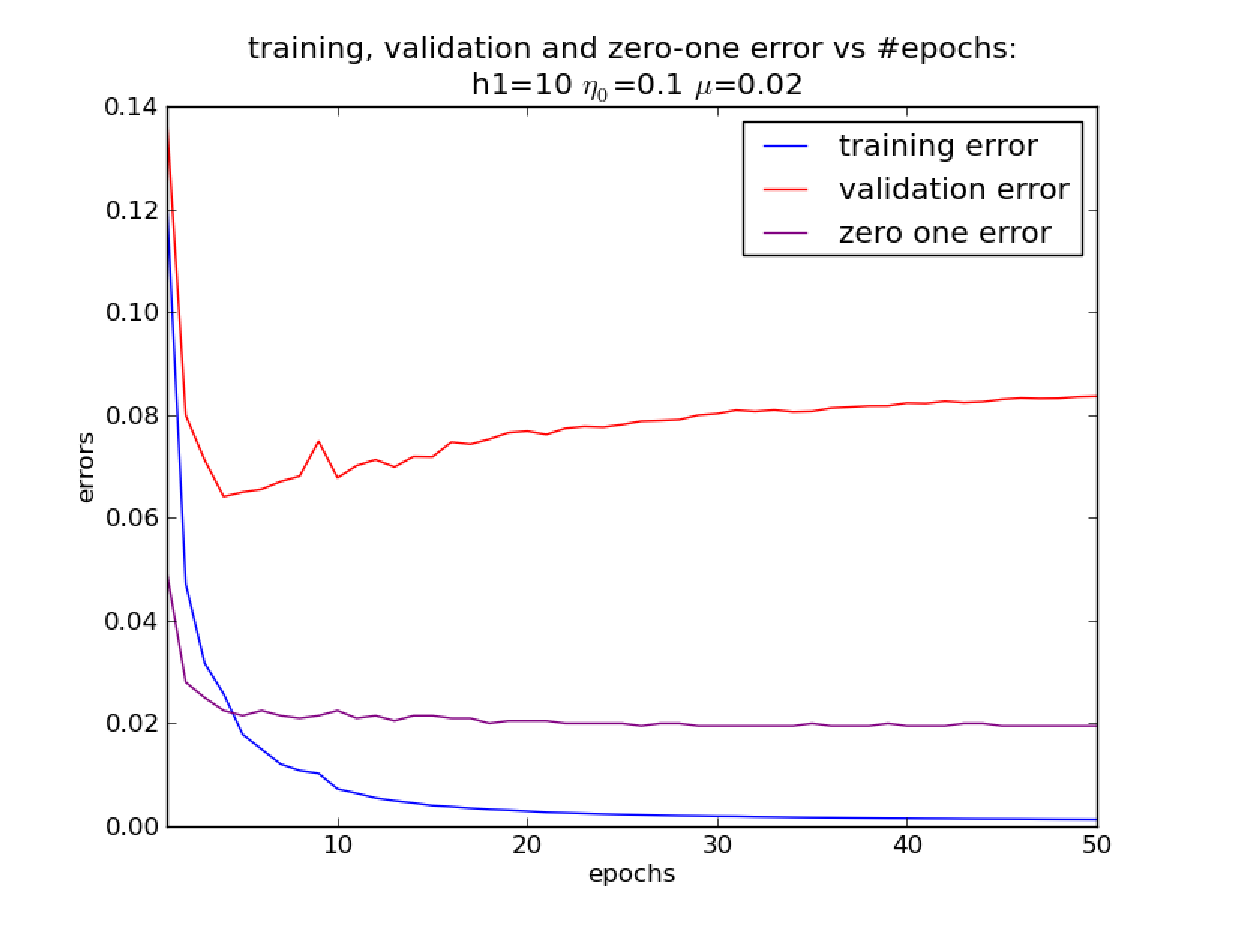
\includegraphics[width=\textwidth]{mlp/plots/test/10h1_overfitting_50_epochs_mu002.eps}
	\caption{}
	\label{subfig:overfit2}
	\end{subfigure}
	\quad	
	\begin{subfigure}[b]{.45\textwidth}
	\centering
	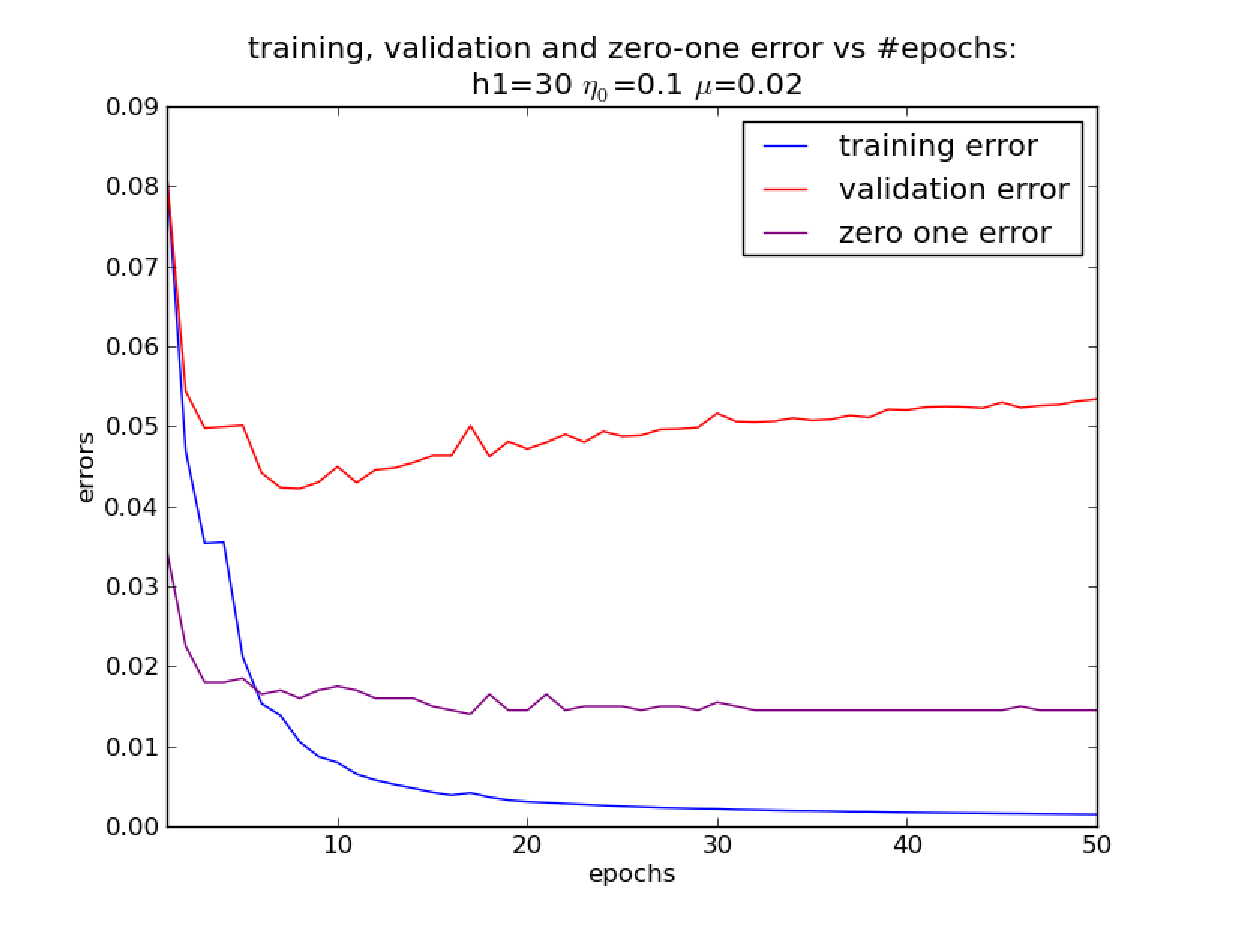
\includegraphics[width=\textwidth]{mlp/plots/test/30h1_overfitting_50_epochs.eps}
	\caption{}
	\label{subfig:overfit3}
	\end{subfigure}
	\quad
	\begin{subfigure}[b]{.45\textwidth}
	\centering
	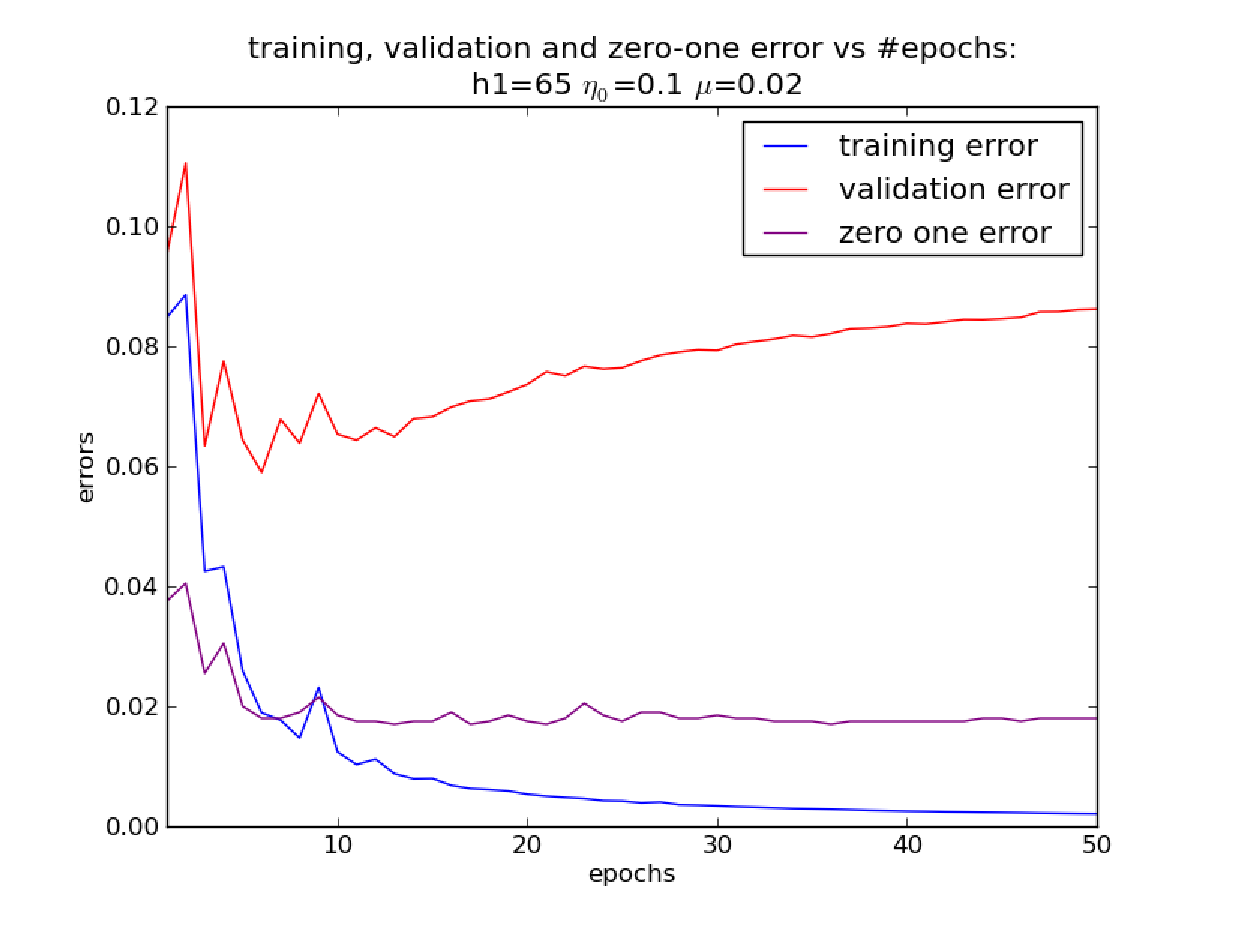
\includegraphics[width=\textwidth]{mlp/plots/test/65h1_overfitting_50_epochs.eps}
	\caption{}
	\label{subfig:overfit4}
	\end{subfigure}
	\caption{Example examples of overfitting for different numbers of hidden units}
	\label{fig:overfitting}
	\end{figure}
In this section we show examples of overfitting through changing the number of hidden units. We expected the validation error to increase more drastically over the number of epochs, while the training error decreases, for higher numbers of hidden units. However, we see in fig. \ref{subfig:overfit1} and fig. \ref{subfig:overfit2} that the result can already be very different for the same parameters. Additionally, for $h_1=30$ in fig. \ref{subfig:overfit3} the effect of overfitting does not appear to be more obvious than in the case of $h_1=10$. Finally we see that with 65 hidden units (fig. \ref{subfig:overfit4}) the validation error does increase more drastically over the 50 epochs indicating that with $h1$ around 65 and larger the now more complex network is more prone to overfitting.

\subsection{Results}
	In this section we show the results obtained with the MLP classifier on both the 3/5 and 4/9 digit provided sets of the MNIST dataset and shortly discuss our choice of parameters for the subtasks.
	\subsubsection{Choice of parameters for subtasks and discussion of performance on test set}
	The best result we recorded on the 3/5 problem was a 0/1 error of 1.367\% of a total of 1902 test points (26 in absolute numbers). To achieve this we used the following parameters: $h_1=10$, $\eta _0=0.1$, $\mu =0.015$. We used the same parameters on the 4/9 problem where the best result on the testing set gave 2.26\% misclassifications (45 in absolute numbers). We tried a number of different combinations of parameter values, however this combination consistently gave the best results for validation and testing for our setup.  
	\begin{figure}[!ht]
	\centering
	\begin{subfigure}[b]{.45\textwidth}
	\centering
	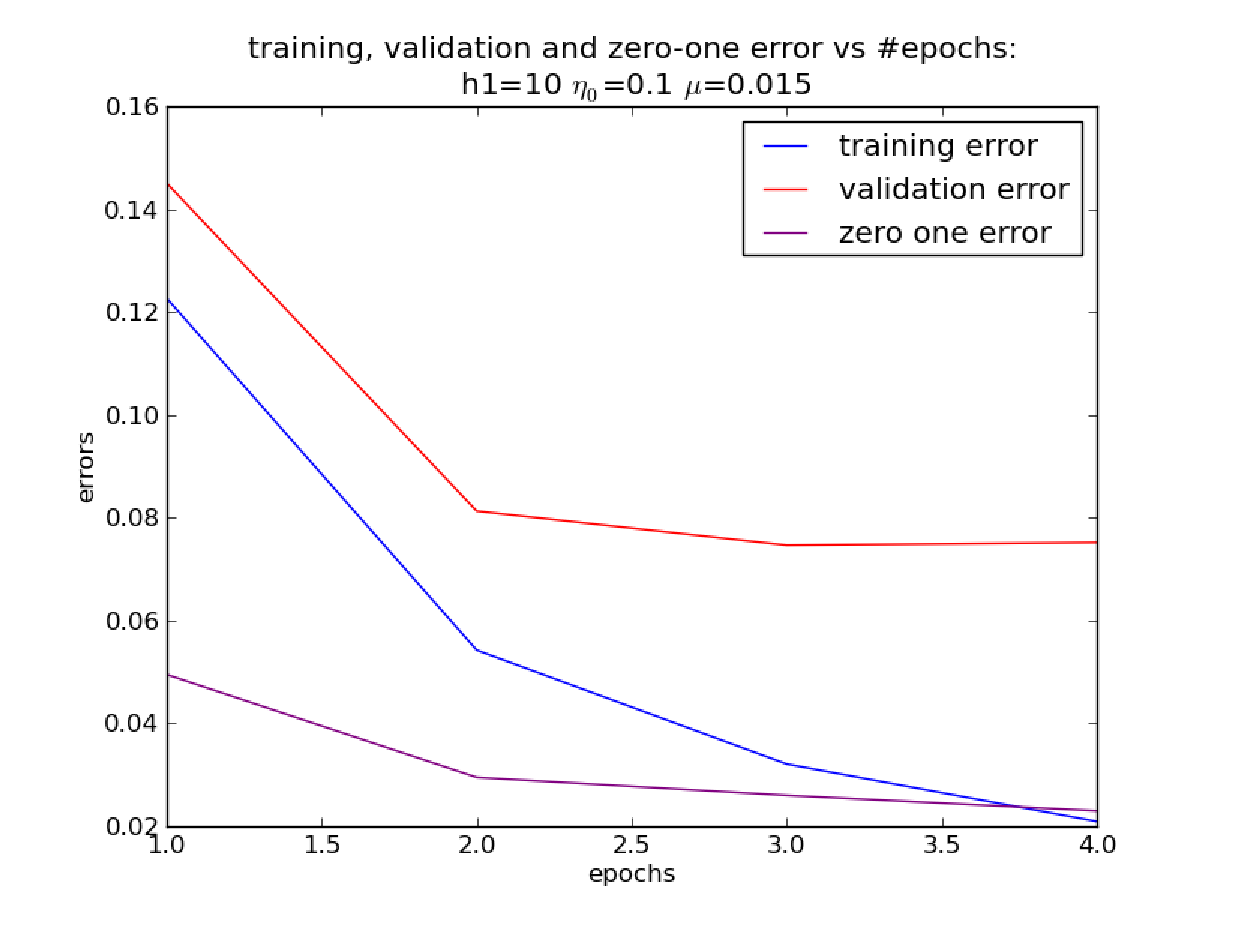
\includegraphics[width=\textwidth]{mlp/plots/3_5/sample.eps}
	\caption{Sample graph for \textbf{mean} 0/1 error on 3/5 testset recorded over 10 runs $0.01845\pm 0.00273$}
	\label{subfig:result3}
	\end{subfigure}
	\quad
	\begin{subfigure}[b]{.45\textwidth}
	\centering
	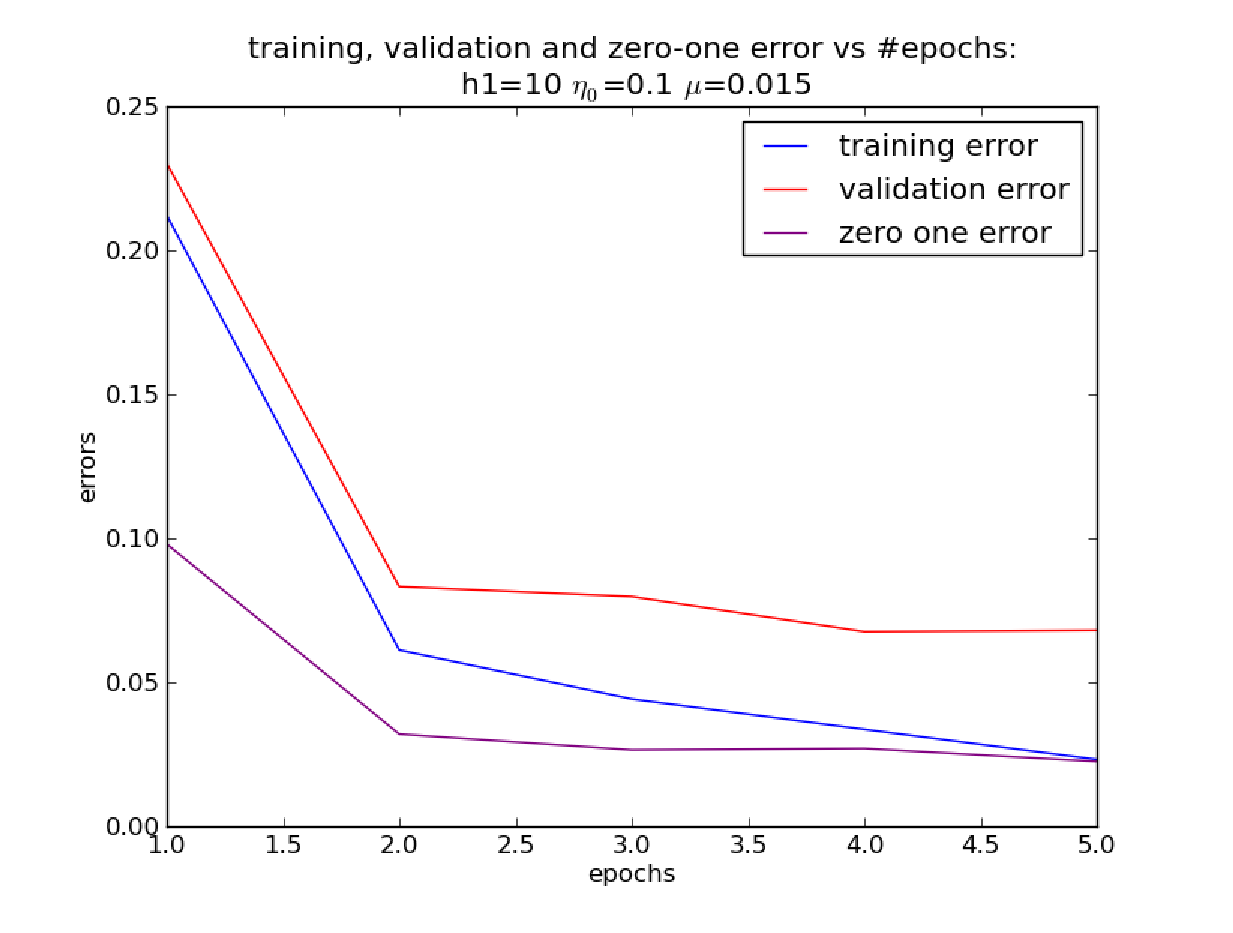
\includegraphics[width=\textwidth]{mlp/plots/4_9/sample.eps}
	\caption{Sample graph for \textbf{mean} 0/1 error on 4/9 testset recorded over 10 runs $0.02395\pm 0.00140$}
	\label{subfig:result4}
	\end{subfigure}
	\caption{Sample graphs of a run of the final parametrization of the MLP on both subtasks annotated with the performance of test with mean and standard deviation}
	\label{fig:performance_result}
	\end{figure}

	\subsubsection{Misclassified patterns}
	Fig. \ref{subfig:misclass_3} shows a misclassified pattern where $t_i a^{(2)}(x_i)<0$ is close to 0. Its actual label is -1, meaning that the data pattern represents a 9. The fact that is was misclassified by little means that the model finds it slightly more similar to a 4 than to its actual value.
	\begin{figure}[!ht]
	\centering
	\begin{subfigure}[b]{.45\textwidth}
	\centering
	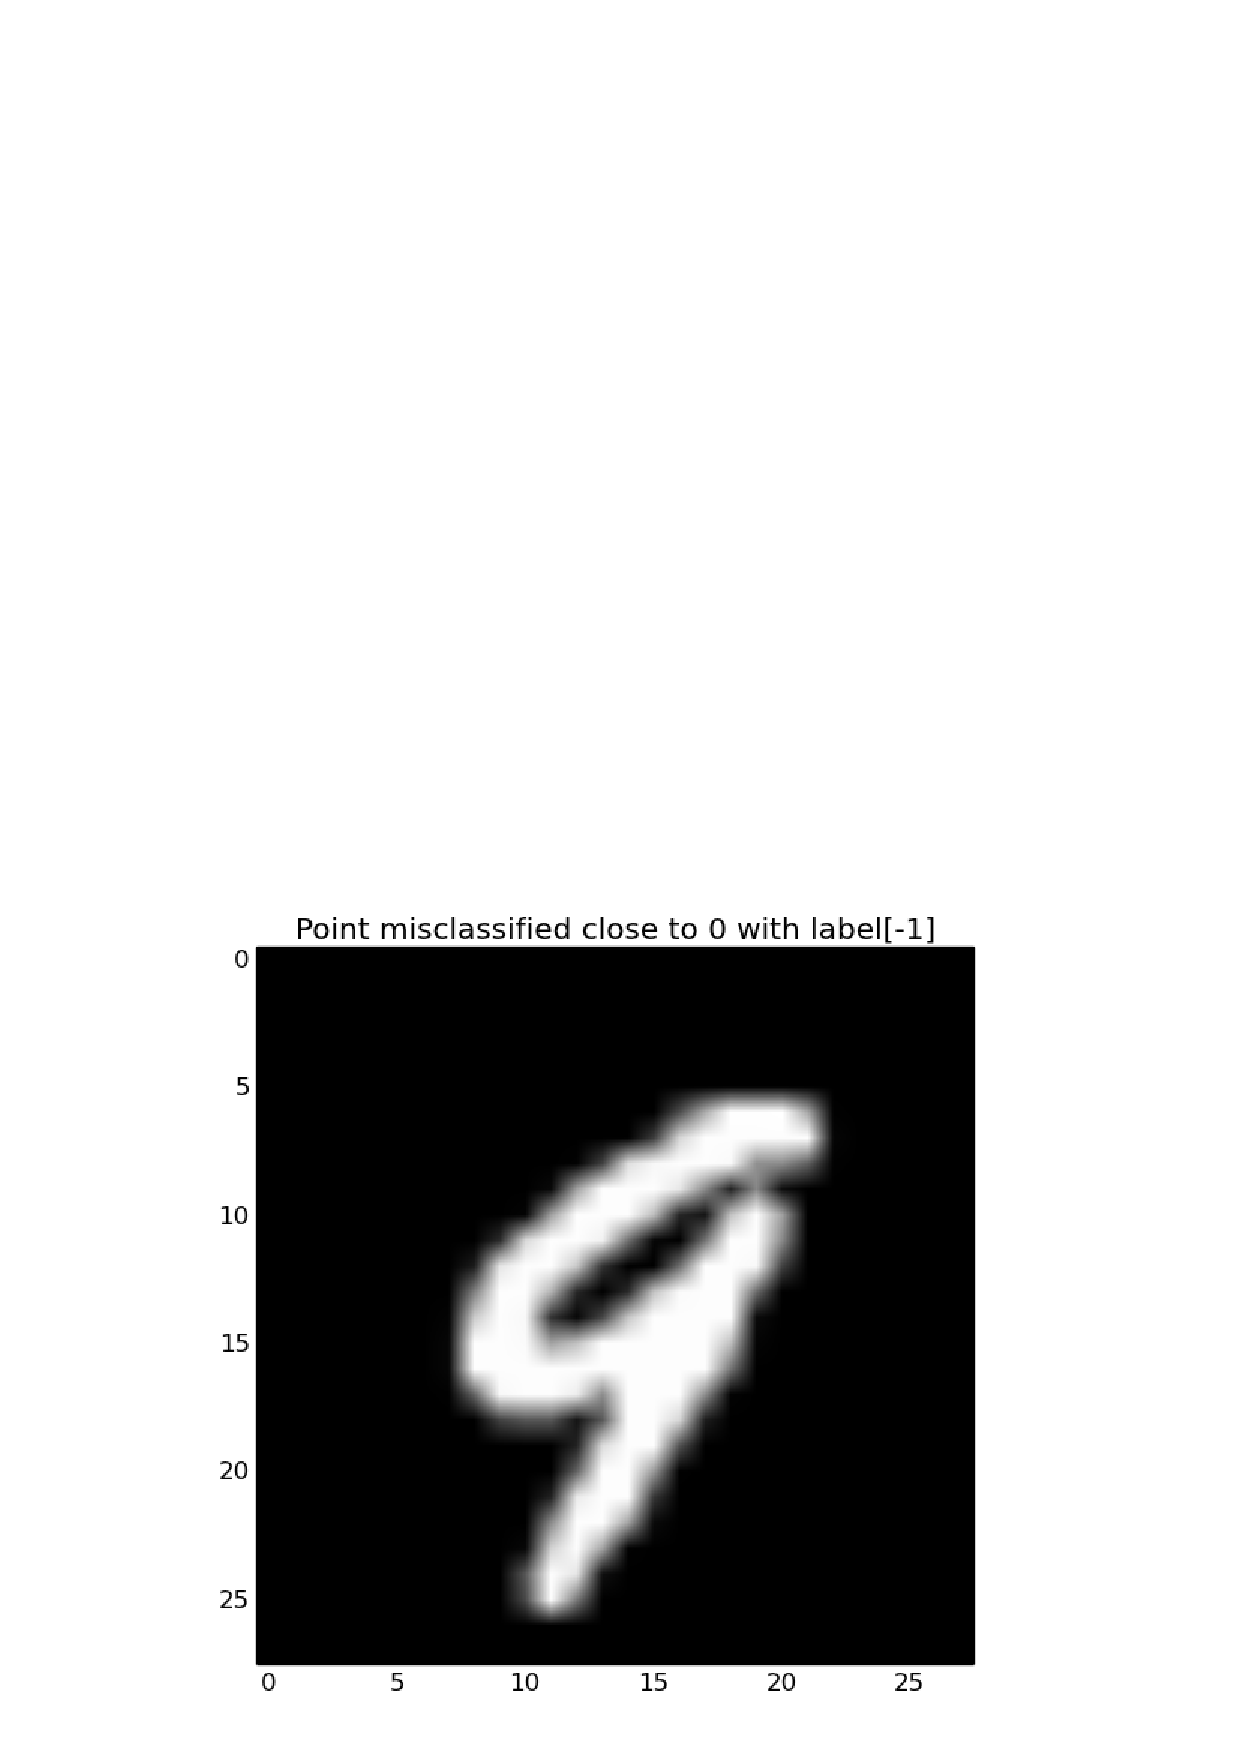
\includegraphics[width=\textwidth]{mlp/plots/misclassified_fig3.png}
	\caption{Binary image of a 9 digit just about misclassified as a 4}
	\label{subfig:misclass_3}
	\end{subfigure}
	\quad
	\begin{subfigure}[b]{.45\textwidth}
	\centering
	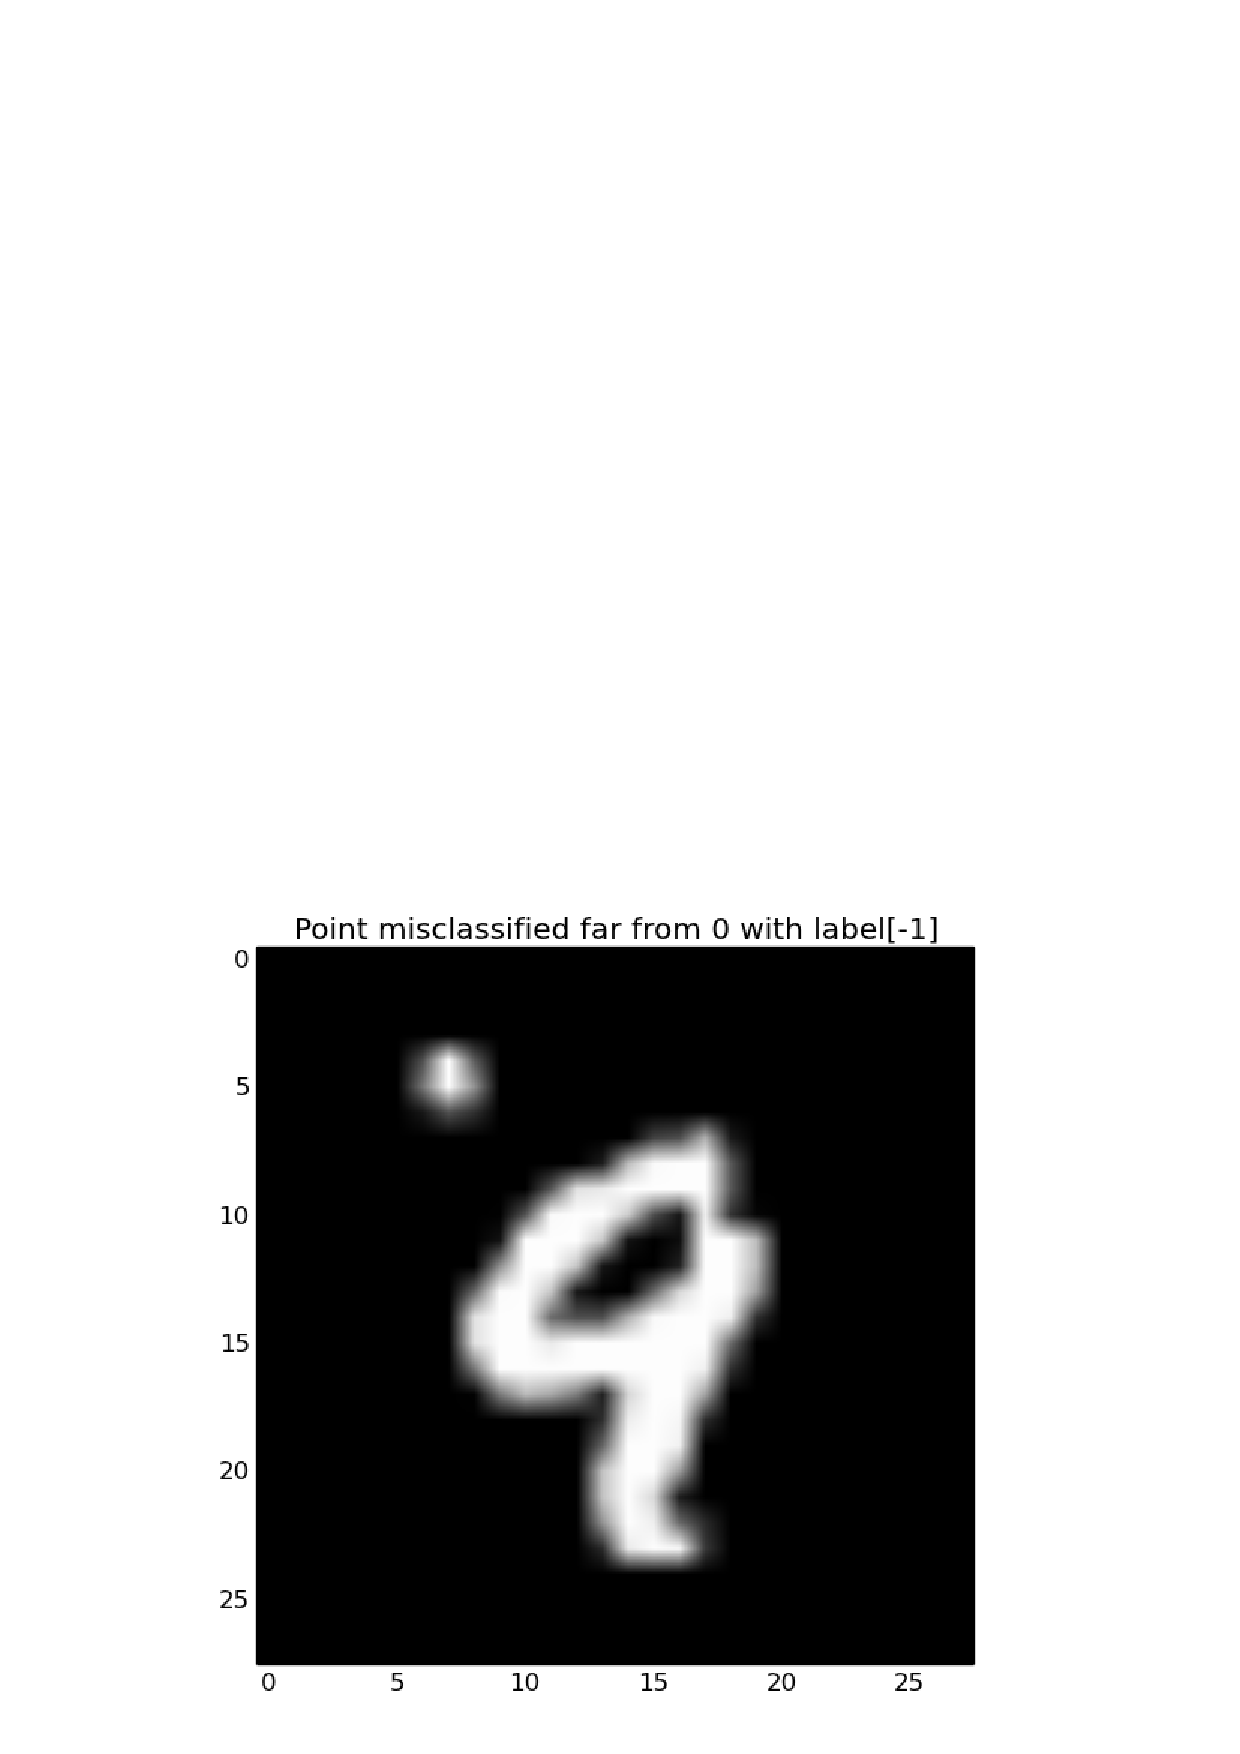
\includegraphics[width=\textwidth]{mlp/plots/misclassified_fig4.png}
	\caption{Binary image of a 9 digit \textbf{clearly} mistaken to be a 4 by the classifier}
	\label{subfig:misclass_4}
	\end{subfigure}
	\caption{Examples of misclassified patterns for the 4-9 problem}
	\label{fig:misclassification}
	\end{figure}
	Fig. \ref{subfig:misclass_4} shows a misclassified point where $t_i a^{(2)}(x_i)<0$ is far from 0. Its actual label is again -1, yet the fact that $a^{(2)}(x_i)a$ was greater than zero means the classifier sees it as a clear 4, assigning it the label 1. That means that in a feature space created from the data patterns the pattern would be an outlier of the "9 class" located in close proximity to patterns of the "4 class".

